% Für Bindekorrektur als optionales Argument "BCORfaktormitmaßeinheit", dann
% sieht auch Option "twoside" vernünftig aus
% Näheres zu "scrartcl" bzw. "scrreprt" und "scrbook" siehe KOMA-Skript Doku
\documentclass[12pt,a4paper,titlepage,headinclude,bibtotoc]{scrartcl}


%---- Allgemeine Layout Einstellungen ------------------------------------------

% Für Kopf und Fußzeilen, siehe auch KOMA-Skript Doku
\usepackage[komastyle]{scrpage2}
\pagestyle{scrheadings}
\automark[section]{chapter}
\setheadsepline{0.5pt}[\color{black}]


%Einstellungen für Figuren- und Tabellenbeschriftungen
\setkomafont{captionlabel}{\sffamily\bfseries}
\setcapindent{0em}


%---- Weitere Pakete -----------------------------------------------------------
% Die Pakete sind alle in der TeX Live Distribution enthalten. Wichtige Adressen
% www.ctan.org, www.dante.de

% Sprachunterstützung
\usepackage[ngerman]{babel}

% Benutzung von Umlauten direkt im Text
% entweder "latin1" oder "utf8"
\usepackage[utf8]{inputenc}

% Pakete mit Mathesymbolen und zur Beseitigung von Schwächen der Mathe-Umgebung
\usepackage{latexsym,exscale,amssymb,amsmath}

% Weitere Symbole
\usepackage[nointegrals]{wasysym}
\usepackage{eurosym}

% Anderes Literaturverzeichnisformat
%\usepackage[square,sort&compress]{natbib}

% Für Farbe
\usepackage{color}

% Zur Graphikausgabe
%Beipiel: \includegraphics[width=\textwidth]{grafik.png}
\usepackage{graphicx}

% Text umfließt Graphiken und Tabellen
% Beispiel:
% \begin{wrapfigure}[Zeilenanzahl]{"l" oder "r"}{breite}
%   \centering
%   \includegraphics[width=...]{grafik}
%   \caption{Beschriftung} 
%   \label{fig:grafik}
% \end{wrapfigure}
\usepackage{wrapfig}

% Mehrere Abbildungen nebeneinander
% Beispiel:
% \begin{figure}[htb]
%   \centering
%   \subfigure[Beschriftung 1\label{fig:label1}]
%   {\includegraphics[width=0.49\textwidth]{grafik1}}
%   \hfill
%   \subfigure[Beschriftung 2\label{fig:label2}]
%   {\includegraphics[width=0.49\textwidth]{grafik2}}
%   \caption{Beschriftung allgemein}
%   \label{fig:label-gesamt}
% \end{figure}
\usepackage{subfigure}

% Caption neben Abbildung
% Beispiel:
% \sidecaptionvpos{figure}{"c" oder "t" oder "b"}
% \begin{SCfigure}[rel. Breite (normalerweise = 1)][hbt]
%   \centering
%   \includegraphics[width=0.5\textwidth]{grafik.png}
%   \caption{Beschreibung}
%   \label{fig:}
% \end{SCfigure}
\usepackage{sidecap}

% Befehl für "Entspricht"-Zeichen
\newcommand{\corresponds}{\ensuremath{\mathrel{\widehat{=}}}}

%Für chemische Formeln (von www.dante.de)
%% Anpassung an LaTeX(2e) von Bernd Raichle
\makeatletter
\DeclareRobustCommand{\chemical}[1]{%
  {\(\m@th
   \edef\resetfontdimens{\noexpand\)%
       \fontdimen16\textfont2=\the\fontdimen16\textfont2
       \fontdimen17\textfont2=\the\fontdimen17\textfont2\relax}%
   \fontdimen16\textfont2=2.7pt \fontdimen17\textfont2=2.7pt
   \mathrm{#1}%
   \resetfontdimens}}
\makeatother

%Si Einheiten
\usepackage{siunitx}

%c++ Code einbinden
\usepackage{listings}
\lstset{numbers=left, numberstyle=\tiny, numbersep=5pt}

%errorFkt
\newcommand{\erf}{\ensuremath{\text{erf}}}

%Boxen,etc.
\usepackage{fancybox}
\usepackage{empheq}

\begin{document}

\begin{titlepage}
\centering
\textsc{\Large Anfängerpraktikum der Fakultät für
  Physik,\\[1.5ex] Universität Göttingen}

\vspace*{4.2cm}

\rule{\textwidth}{1pt}\\[0.5cm]
{\huge \bfseries
  Diffusion\\[1.5ex]
  Protokoll:}\\[0.5cm]
\rule{\textwidth}{1pt}

\vspace*{3.0cm}

\begin{Large}
\begin{tabular}{ll}
Praktikant:
%	&  Skrollan Detzler\\
 	&  Felix Kurtz\\
% 	&  Michael Lohmann\\
%	&  Kevin Lüdemann\\

  E-Mail: 
%	&  skrollan.detzler@stud.uni-goettingen.de\\
	&  felix.kurtz@stud.uni-goettingen.de\\
%	& m.lohmann@stud.uni-goettingen.de\\
%	&  kevin.luedemann@stud.uni-goettingen.de\\

Versuchspartner:
	&  Skrollan Detzler\\
% 	&  Felix Kurtz\\
% 	&  Michael Lohmann\\
%	&  Kevin Lüdemann\\

 Betreuer: & Martin Ochmann\\
 Versuchsdatum: & 30.06.2014\\
\end{tabular}
\end{Large}

\vspace*{0.8cm}

\begin{Large}
\fbox{
  \begin{minipage}[t][2.5cm][t]{6cm} 
    Note:
  \end{minipage}
}
\end{Large}

\end{titlepage}

\tableofcontents

\newpage

\section{Einleitung}
\label{sec:einleitung}
In diesem Versuch soll das Phänomen der \textit{Diffusion} untersucht werden.
Darunter versteht man die Durchmischung von zwei verschiedenen Gasen oder Flüssigkeiten, welche mit der Zeit vonstatten geht.
Sie spielt besonders in der Biologie bei osmotischen Prozessen eine große Rolle.
Als eine von vielen Transportphänomenen wie Wärmeleitung ist sie jedoch am besten experimentell messbar.\\
Wir wollen hier die Diffusion von Methylenblau in Wasser untersuchen.

\section{Theorie}
\label{sec:theorie}
\subsection{Ficksche Gesetze}
\textbf{1.Ficksches Gesetz}
\begin{empheq}[box=\shadowbox*]{align}
\vec{j}(\vec{x})=-D\cdot\nabla n
\end{empheq}
\textbf{2.Ficksches Gesetz}
\begin{empheq}[box=\shadowbox*]{align}
\frac{\partial n}{\partial t}=-D\cdot\Delta n
\end{empheq}

Man kann dies analytisch lösen. Dabei ergibt sich dies als Lösung:
\begin{align}
	c(x,t)=\frac{c_0}{2} \left[1-\erf\left(\frac{x}{\sqrt{4Dt}}\right)\right]	
	\label{eq:DiffLsg}
\end{align}
Gaußsche Fehlerfunktion
\begin{align*}
	\erf(y):=\frac{2}{\sqrt{\pi}} \int_0^y \! e^{-v^2}\, \mathrm{d}v
\end{align*}

\subsection{Wheatstone'sche Messbrücke}
\begin{figure}[!htb]
	\centering	
	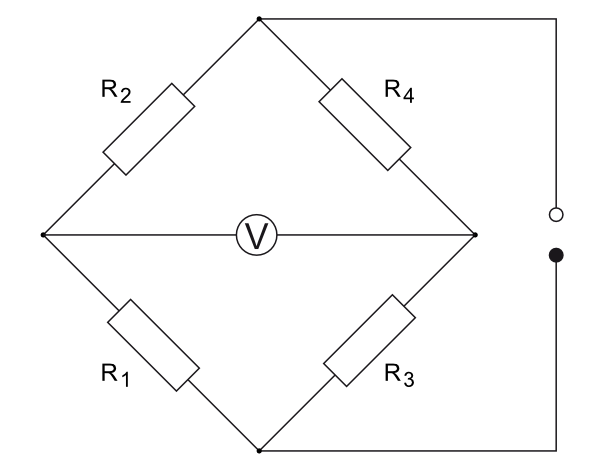
\includegraphics[scale=0.7]{Brueckenschaltung.png}
	\caption{Wheatstone'sche Brückenschaltung \cite{lp}}
\end{figure}


\section{Durchführung}
\label{sec:durchfuehrung}
\subsection{Versuchsaufbau}
\begin{figure}[!htb]
	\centering	
	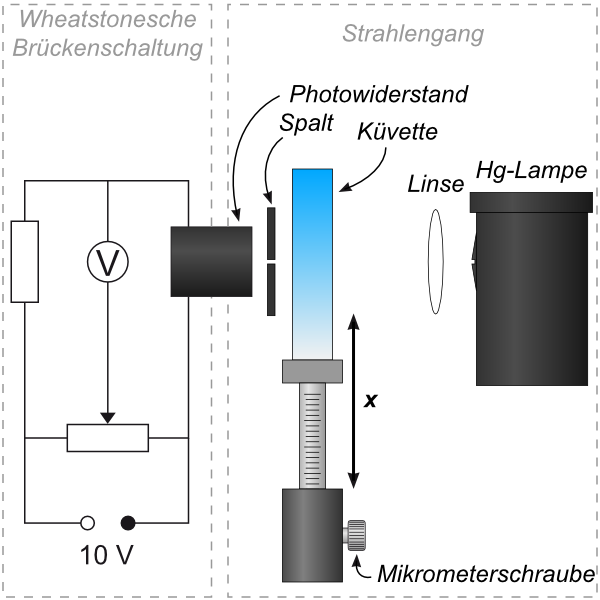
\includegraphics[scale=0.7]{Aufbau_schematisch.png}
	\caption{schematischer Versuchsaufbau \cite{lp}}
\end{figure}
Zuerst wird der Spalt so justiert, dass auf den Photowiderstand die maximale Intensität trifft.
Außerdem benötigt man noch zwei Stoppuhren für die späteren Messungen.
\subsection{Konzentrationsverlauf in Abhängigkeit der Zeit}
Für den Graufilter $c_0/16$ regelt man das Potentiometer so, dass das Amperemeter keinen Strom anzeigt.
Dann wird die Küvette zu $3/4$ mit Wasser gefüllt, darüber Methylenblau.
Man startet die Stoppuhr, nachdem man die Küvette in den Strahlengang gestellt hat.
Für eine halbe Stunde notiert man alle 30 Sekunden den Ort der Konzentration $c_0/16$.
Dabei wird jedoch die Messbrücke nicht verändert, sondern die Küvette mittels Micrometerschraube nach oben bewegt, bis das Amperemeter wieder keinen Strom zeigt.\\
Nach der Messung wird diese Küvette vorsichtig zur Seite gestellt, damit sich die Flüssigkeiten nicht zusätzlich vermischen.
Die benutzte Stoppuhr lässt man für eine spätere Messung weiterlaufen.
Dann füllt man eine zweite Küvette wie die erste, gleicht aber die Messbrücke mit dem Graufilter $c_0/32$ ab.
Die vorige Messung wird mit der zweiten Küvette, der zweiten Stoppuhr und dem anderen Filter wiederholt.
\subsection{Konzentrationsprofil}
Etwa 40 Minuten nach Beginn der letzten Messung wird die Konzentrationsverteilug der zweiten Küvette in Abhängigkeit des Ortes gemessen.
Dies sollte schnell geschehen, damit die Zeit als konstant angenommen werden kann.
Trotzdem notiert man Beginn und Ende dieser Messung, die Stoppuhr muss also weiter laufen.
Der Messvorgang sieht folgendermaßen aus:
Nacheinander wird die Messbrücke auf die verschiedenen Graufilter $c_0/2, c_0/4, c_0/8, c_0/16, c_0/32$ abgeglichen, bevor man dazu die Stelle sucht, an der genau diese Konzentration herrscht.
Diesen Vorgang wiederholt man nochmal in umgekehrter Reihenfolge der Graufilter.\\
Diesen ganzen Messvorgang wird für die erste Küvette nach ca. 100 Minuten  seit Beginn der zugehörigen ersten Messung wiederholt. 

\section{Auswertung}
\label{sec:auswertung}

\subsection{erwartete Diffusionskurven}
\begin{figure}
	% GNUPLOT: LaTeX picture with Postscript
\begingroup
  \makeatletter
  \providecommand\color[2][]{%
    \GenericError{(gnuplot) \space\space\space\@spaces}{%
      Package color not loaded in conjunction with
      terminal option `colourtext'%
    }{See the gnuplot documentation for explanation.%
    }{Either use 'blacktext' in gnuplot or load the package
      color.sty in LaTeX.}%
    \renewcommand\color[2][]{}%
  }%
  \providecommand\includegraphics[2][]{%
    \GenericError{(gnuplot) \space\space\space\@spaces}{%
      Package graphicx or graphics not loaded%
    }{See the gnuplot documentation for explanation.%
    }{The gnuplot epslatex terminal needs graphicx.sty or graphics.sty.}%
    \renewcommand\includegraphics[2][]{}%
  }%
  \providecommand\rotatebox[2]{#2}%
  \@ifundefined{ifGPcolor}{%
    \newif\ifGPcolor
    \GPcolortrue
  }{}%
  \@ifundefined{ifGPblacktext}{%
    \newif\ifGPblacktext
    \GPblacktexttrue
  }{}%
  % define a \g@addto@macro without @ in the name:
  \let\gplgaddtomacro\g@addto@macro
  % define empty templates for all commands taking text:
  \gdef\gplbacktext{}%
  \gdef\gplfronttext{}%
  \makeatother
  \ifGPblacktext
    % no textcolor at all
    \def\colorrgb#1{}%
    \def\colorgray#1{}%
  \else
    % gray or color?
    \ifGPcolor
      \def\colorrgb#1{\color[rgb]{#1}}%
      \def\colorgray#1{\color[gray]{#1}}%
      \expandafter\def\csname LTw\endcsname{\color{white}}%
      \expandafter\def\csname LTb\endcsname{\color{black}}%
      \expandafter\def\csname LTa\endcsname{\color{black}}%
      \expandafter\def\csname LT0\endcsname{\color[rgb]{1,0,0}}%
      \expandafter\def\csname LT1\endcsname{\color[rgb]{0,1,0}}%
      \expandafter\def\csname LT2\endcsname{\color[rgb]{0,0,1}}%
      \expandafter\def\csname LT3\endcsname{\color[rgb]{1,0,1}}%
      \expandafter\def\csname LT4\endcsname{\color[rgb]{0,1,1}}%
      \expandafter\def\csname LT5\endcsname{\color[rgb]{1,1,0}}%
      \expandafter\def\csname LT6\endcsname{\color[rgb]{0,0,0}}%
      \expandafter\def\csname LT7\endcsname{\color[rgb]{1,0.3,0}}%
      \expandafter\def\csname LT8\endcsname{\color[rgb]{0.5,0.5,0.5}}%
    \else
      % gray
      \def\colorrgb#1{\color{black}}%
      \def\colorgray#1{\color[gray]{#1}}%
      \expandafter\def\csname LTw\endcsname{\color{white}}%
      \expandafter\def\csname LTb\endcsname{\color{black}}%
      \expandafter\def\csname LTa\endcsname{\color{black}}%
      \expandafter\def\csname LT0\endcsname{\color{black}}%
      \expandafter\def\csname LT1\endcsname{\color{black}}%
      \expandafter\def\csname LT2\endcsname{\color{black}}%
      \expandafter\def\csname LT3\endcsname{\color{black}}%
      \expandafter\def\csname LT4\endcsname{\color{black}}%
      \expandafter\def\csname LT5\endcsname{\color{black}}%
      \expandafter\def\csname LT6\endcsname{\color{black}}%
      \expandafter\def\csname LT7\endcsname{\color{black}}%
      \expandafter\def\csname LT8\endcsname{\color{black}}%
    \fi
  \fi
  \setlength{\unitlength}{0.0500bp}%
  \begin{picture}(7200.00,5040.00)%
    \gplgaddtomacro\gplbacktext{%
      \csname LTb\endcsname%
      \put(1254,1043){\makebox(0,0)[r]{\strut{} 0}}%
      \put(1254,1722){\makebox(0,0)[r]{\strut{} 0.2}}%
      \put(1254,2401){\makebox(0,0)[r]{\strut{} 0.4}}%
      \put(1254,3079){\makebox(0,0)[r]{\strut{} 0.6}}%
      \put(1254,3758){\makebox(0,0)[r]{\strut{} 0.8}}%
      \put(1254,4437){\makebox(0,0)[r]{\strut{} 1}}%
      \put(1943,484){\makebox(0,0){\strut{}-4}}%
      \put(3058,484){\makebox(0,0){\strut{}-2}}%
      \put(4172,484){\makebox(0,0){\strut{} 0}}%
      \put(5286,484){\makebox(0,0){\strut{} 2}}%
      \put(6401,484){\makebox(0,0){\strut{} 4}}%
      \put(484,2740){\rotatebox{90}{\makebox(0,0){\strut{}$c(x,t)/c_0$}}}%
      \put(4172,154){\makebox(0,0){\strut{}$x$ [mm]}}%
    }%
    \gplgaddtomacro\gplfronttext{%
      \put(5971,4603){\makebox(0,0)[r]{\strut{}$t=0$}}%
      \csname LTb\endcsname%
      \put(5971,4383){\makebox(0,0)[r]{\strut{}$t=30~\si{\minute}$}}%
      \csname LTb\endcsname%
      \put(5971,4163){\makebox(0,0)[r]{\strut{}$t=90~\si{\minute}$}}%
      \csname LTb\endcsname%
      \put(5971,3943){\makebox(0,0)[r]{\strut{}$t=6~\si{\hour}$}}%
      \csname LTb\endcsname%
      \put(5971,3723){\makebox(0,0)[r]{\strut{}$t=2~\si{\day}$}}%
    }%
    \gplbacktext
    \put(0,0){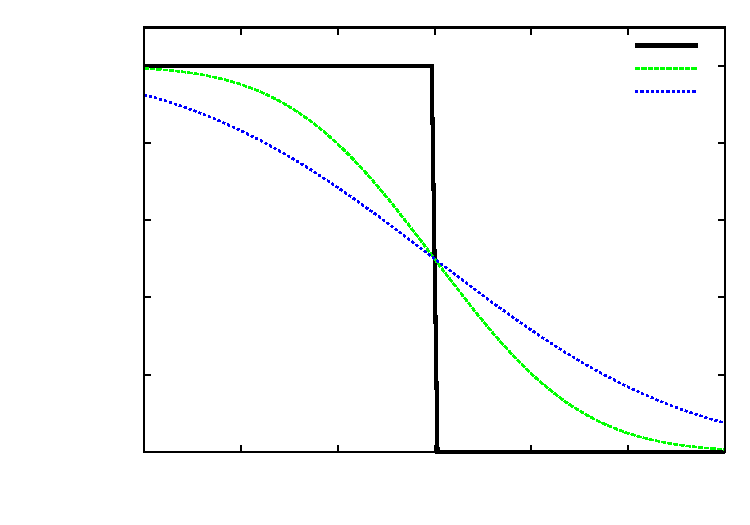
\includegraphics{errorfkt}}%
    \gplfronttext
  \end{picture}%
\endgroup

	\caption{Profil für den Diffusionskoeffizienten $D=4\cdot 10^{-10} ~ \si{\meter ^2 / \second}$ zu verschiedenen Zeiten}
	\label{fig:erwDiffKurve}
\end{figure}

Aus der Lösung der Diffusionsgleichung \eqref{eq:DiffLsg} ergibt sich Abbildung \ref{fig:erwDiffKurve}.
Man erkennt,dass es zu $t=0$ eine klare Grenze zwischen den beiden Flüssigkeiten.
Im Verlauf der Zeit (hier nach 30 und 90 Minuten) vermischen sie sich.
Bei $x=0$ befindet sich jedoch immer die Konzentration $c_0/2$.

\subsection{Berechnung des Diffusionskoeefizienten}

\begin{figure}
	% GNUPLOT: LaTeX picture with Postscript
\begingroup
  \makeatletter
  \providecommand\color[2][]{%
    \GenericError{(gnuplot) \space\space\space\@spaces}{%
      Package color not loaded in conjunction with
      terminal option `colourtext'%
    }{See the gnuplot documentation for explanation.%
    }{Either use 'blacktext' in gnuplot or load the package
      color.sty in LaTeX.}%
    \renewcommand\color[2][]{}%
  }%
  \providecommand\includegraphics[2][]{%
    \GenericError{(gnuplot) \space\space\space\@spaces}{%
      Package graphicx or graphics not loaded%
    }{See the gnuplot documentation for explanation.%
    }{The gnuplot epslatex terminal needs graphicx.sty or graphics.sty.}%
    \renewcommand\includegraphics[2][]{}%
  }%
  \providecommand\rotatebox[2]{#2}%
  \@ifundefined{ifGPcolor}{%
    \newif\ifGPcolor
    \GPcolortrue
  }{}%
  \@ifundefined{ifGPblacktext}{%
    \newif\ifGPblacktext
    \GPblacktexttrue
  }{}%
  % define a \g@addto@macro without @ in the name:
  \let\gplgaddtomacro\g@addto@macro
  % define empty templates for all commands taking text:
  \gdef\gplbacktext{}%
  \gdef\gplfronttext{}%
  \makeatother
  \ifGPblacktext
    % no textcolor at all
    \def\colorrgb#1{}%
    \def\colorgray#1{}%
  \else
    % gray or color?
    \ifGPcolor
      \def\colorrgb#1{\color[rgb]{#1}}%
      \def\colorgray#1{\color[gray]{#1}}%
      \expandafter\def\csname LTw\endcsname{\color{white}}%
      \expandafter\def\csname LTb\endcsname{\color{black}}%
      \expandafter\def\csname LTa\endcsname{\color{black}}%
      \expandafter\def\csname LT0\endcsname{\color[rgb]{1,0,0}}%
      \expandafter\def\csname LT1\endcsname{\color[rgb]{0,1,0}}%
      \expandafter\def\csname LT2\endcsname{\color[rgb]{0,0,1}}%
      \expandafter\def\csname LT3\endcsname{\color[rgb]{1,0,1}}%
      \expandafter\def\csname LT4\endcsname{\color[rgb]{0,1,1}}%
      \expandafter\def\csname LT5\endcsname{\color[rgb]{1,1,0}}%
      \expandafter\def\csname LT6\endcsname{\color[rgb]{0,0,0}}%
      \expandafter\def\csname LT7\endcsname{\color[rgb]{1,0.3,0}}%
      \expandafter\def\csname LT8\endcsname{\color[rgb]{0.5,0.5,0.5}}%
    \else
      % gray
      \def\colorrgb#1{\color{black}}%
      \def\colorgray#1{\color[gray]{#1}}%
      \expandafter\def\csname LTw\endcsname{\color{white}}%
      \expandafter\def\csname LTb\endcsname{\color{black}}%
      \expandafter\def\csname LTa\endcsname{\color{black}}%
      \expandafter\def\csname LT0\endcsname{\color{black}}%
      \expandafter\def\csname LT1\endcsname{\color{black}}%
      \expandafter\def\csname LT2\endcsname{\color{black}}%
      \expandafter\def\csname LT3\endcsname{\color{black}}%
      \expandafter\def\csname LT4\endcsname{\color{black}}%
      \expandafter\def\csname LT5\endcsname{\color{black}}%
      \expandafter\def\csname LT6\endcsname{\color{black}}%
      \expandafter\def\csname LT7\endcsname{\color{black}}%
      \expandafter\def\csname LT8\endcsname{\color{black}}%
    \fi
  \fi
  \setlength{\unitlength}{0.0500bp}%
  \begin{picture}(7200.00,5040.00)%
    \gplgaddtomacro\gplbacktext{%
      \csname LTb\endcsname%
      \put(1254,704){\makebox(0,0)[r]{\strut{} 0}}%
      \put(1254,1156){\makebox(0,0)[r]{\strut{} 0.5}}%
      \put(1254,1609){\makebox(0,0)[r]{\strut{} 1}}%
      \put(1254,2061){\makebox(0,0)[r]{\strut{} 1.5}}%
      \put(1254,2514){\makebox(0,0)[r]{\strut{} 2}}%
      \put(1254,2966){\makebox(0,0)[r]{\strut{} 2.5}}%
      \put(1254,3419){\makebox(0,0)[r]{\strut{} 3}}%
      \put(1254,3871){\makebox(0,0)[r]{\strut{} 3.5}}%
      \put(1254,4324){\makebox(0,0)[r]{\strut{} 4}}%
      \put(1254,4776){\makebox(0,0)[r]{\strut{} 4.5}}%
      \put(1386,484){\makebox(0,0){\strut{} 0}}%
      \put(2005,484){\makebox(0,0){\strut{} 200}}%
      \put(2624,484){\makebox(0,0){\strut{} 400}}%
      \put(3243,484){\makebox(0,0){\strut{} 600}}%
      \put(3862,484){\makebox(0,0){\strut{} 800}}%
      \put(4482,484){\makebox(0,0){\strut{} 1000}}%
      \put(5101,484){\makebox(0,0){\strut{} 1200}}%
      \put(5720,484){\makebox(0,0){\strut{} 1400}}%
      \put(6339,484){\makebox(0,0){\strut{} 1600}}%
      \put(6958,484){\makebox(0,0){\strut{} 1800}}%
      \put(484,2740){\rotatebox{90}{\makebox(0,0){\strut{}Quadrat der Diffusionstrecke [mm$^2$]}}}%
      \put(4172,154){\makebox(0,0){\strut{}Zeit [s]}}%
    }%
    \gplgaddtomacro\gplfronttext{%
      \csname LTb\endcsname%
      \put(4686,4603){\makebox(0,0)[r]{\strut{}Messpunkte c0/16}}%
      \csname LTb\endcsname%
      \put(4686,4383){\makebox(0,0)[r]{\strut{}lineare Regression c0/16}}%
      \csname LTb\endcsname%
      \put(4686,4163){\makebox(0,0)[r]{\strut{}Messpunkte c0/32}}%
      \csname LTb\endcsname%
      \put(4686,3943){\makebox(0,0)[r]{\strut{}lineare Regression c0/32}}%
    }%
    \gplbacktext
    \put(0,0){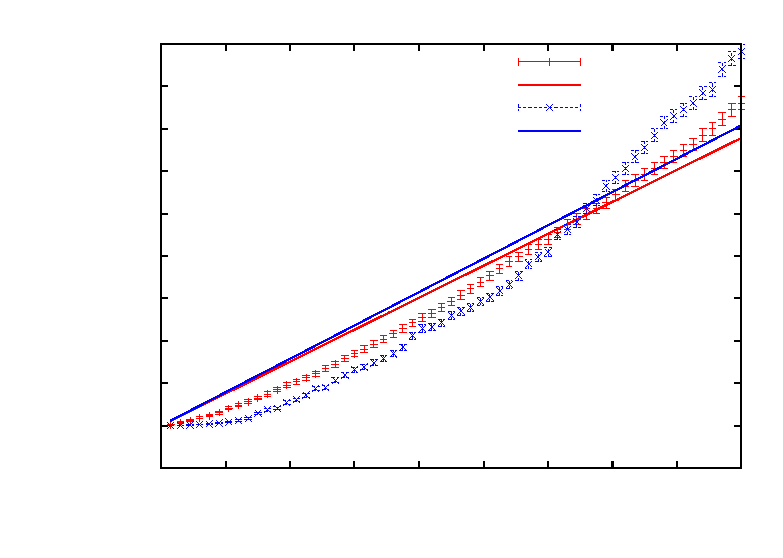
\includegraphics{DiffStrecke}}%
    \gplfronttext
  \end{picture}%
\endgroup

	\caption{???????????????????}
\end{figure}


\begin{align}
	D&=\frac{m}{4~C^2}\\
	\sigma_D&=\frac{\sigma_m}{4~C^2}
\end{align}

\begin{align}
	\erf(y)=\erf\left(\frac{x}{\sqrt{4Dt}}\right)
\end{align}

\begin{table}[!htb]
\centering
\begin{tabular}{|c|c|c|}
	\hline		
	& Messung 1 & Messung 2 \\
	& $c_0/16$ & $c_0/32$ \\
	\hline
	\hline
	y genähert \footnotemark & $1.085$ & $1.317$ \\	
	
	Steigung m & 
	$(18.8 \pm 0.3) \cdot 10^{-10}\si{\meter ^2 / \second}$ & 
	$(19.7 \pm 0.6) \cdot 10^{-10} \si{ \meter ^2 / \second}$ \\	
	
	Diffusionskoeffizient D &
	$(4.00 \pm 0.06) \cdot 10^{-10}\si{\meter ^2 / \second}$ & 
	$(2.83 \pm 0.09) \cdot 10^{-10} \si{ \meter ^2 / \second}$ \\	
	\hline		
\end{tabular}
\caption{Auswertung Messung 1 und 2}
\label{tab:ausw12}
\end{table}

\footnotetext{\textit{WolframAlpha}, www.wolframalpha.com}

\begin{empheq}[box=\shadowbox*]{align}
\overline{D}&=(3.63\pm 0.04) \cdot 10^{-10}\si{ \meter ^2 / \second}
\end{empheq}

\subsection{Konzentrationsprofil}
\begin{figure}
	% GNUPLOT: LaTeX picture with Postscript
\begingroup
  \makeatletter
  \providecommand\color[2][]{%
    \GenericError{(gnuplot) \space\space\space\@spaces}{%
      Package color not loaded in conjunction with
      terminal option `colourtext'%
    }{See the gnuplot documentation for explanation.%
    }{Either use 'blacktext' in gnuplot or load the package
      color.sty in LaTeX.}%
    \renewcommand\color[2][]{}%
  }%
  \providecommand\includegraphics[2][]{%
    \GenericError{(gnuplot) \space\space\space\@spaces}{%
      Package graphicx or graphics not loaded%
    }{See the gnuplot documentation for explanation.%
    }{The gnuplot epslatex terminal needs graphicx.sty or graphics.sty.}%
    \renewcommand\includegraphics[2][]{}%
  }%
  \providecommand\rotatebox[2]{#2}%
  \@ifundefined{ifGPcolor}{%
    \newif\ifGPcolor
    \GPcolortrue
  }{}%
  \@ifundefined{ifGPblacktext}{%
    \newif\ifGPblacktext
    \GPblacktexttrue
  }{}%
  % define a \g@addto@macro without @ in the name:
  \let\gplgaddtomacro\g@addto@macro
  % define empty templates for all commands taking text:
  \gdef\gplbacktext{}%
  \gdef\gplfronttext{}%
  \makeatother
  \ifGPblacktext
    % no textcolor at all
    \def\colorrgb#1{}%
    \def\colorgray#1{}%
  \else
    % gray or color?
    \ifGPcolor
      \def\colorrgb#1{\color[rgb]{#1}}%
      \def\colorgray#1{\color[gray]{#1}}%
      \expandafter\def\csname LTw\endcsname{\color{white}}%
      \expandafter\def\csname LTb\endcsname{\color{black}}%
      \expandafter\def\csname LTa\endcsname{\color{black}}%
      \expandafter\def\csname LT0\endcsname{\color[rgb]{1,0,0}}%
      \expandafter\def\csname LT1\endcsname{\color[rgb]{0,1,0}}%
      \expandafter\def\csname LT2\endcsname{\color[rgb]{0,0,1}}%
      \expandafter\def\csname LT3\endcsname{\color[rgb]{1,0,1}}%
      \expandafter\def\csname LT4\endcsname{\color[rgb]{0,1,1}}%
      \expandafter\def\csname LT5\endcsname{\color[rgb]{1,1,0}}%
      \expandafter\def\csname LT6\endcsname{\color[rgb]{0,0,0}}%
      \expandafter\def\csname LT7\endcsname{\color[rgb]{1,0.3,0}}%
      \expandafter\def\csname LT8\endcsname{\color[rgb]{0.5,0.5,0.5}}%
    \else
      % gray
      \def\colorrgb#1{\color{black}}%
      \def\colorgray#1{\color[gray]{#1}}%
      \expandafter\def\csname LTw\endcsname{\color{white}}%
      \expandafter\def\csname LTb\endcsname{\color{black}}%
      \expandafter\def\csname LTa\endcsname{\color{black}}%
      \expandafter\def\csname LT0\endcsname{\color{black}}%
      \expandafter\def\csname LT1\endcsname{\color{black}}%
      \expandafter\def\csname LT2\endcsname{\color{black}}%
      \expandafter\def\csname LT3\endcsname{\color{black}}%
      \expandafter\def\csname LT4\endcsname{\color{black}}%
      \expandafter\def\csname LT5\endcsname{\color{black}}%
      \expandafter\def\csname LT6\endcsname{\color{black}}%
      \expandafter\def\csname LT7\endcsname{\color{black}}%
      \expandafter\def\csname LT8\endcsname{\color{black}}%
    \fi
  \fi
  \setlength{\unitlength}{0.0500bp}%
  \begin{picture}(7200.00,5040.00)%
    \gplgaddtomacro\gplbacktext{%
      \csname LTb\endcsname%
      \put(1254,704){\makebox(0,0)[r]{\strut{} 0}}%
      \put(1254,1444){\makebox(0,0)[r]{\strut{} 0.1}}%
      \put(1254,2185){\makebox(0,0)[r]{\strut{} 0.2}}%
      \put(1254,2925){\makebox(0,0)[r]{\strut{} 0.3}}%
      \put(1254,3665){\makebox(0,0)[r]{\strut{} 0.4}}%
      \put(1254,4406){\makebox(0,0)[r]{\strut{} 0.5}}%
      \put(1566,484){\makebox(0,0){\strut{} 0}}%
      \put(2464,484){\makebox(0,0){\strut{} 1}}%
      \put(3363,484){\makebox(0,0){\strut{} 2}}%
      \put(4262,484){\makebox(0,0){\strut{} 3}}%
      \put(5161,484){\makebox(0,0){\strut{} 4}}%
      \put(6059,484){\makebox(0,0){\strut{} 5}}%
      \put(6958,484){\makebox(0,0){\strut{} 6}}%
      \put(484,2740){\rotatebox{90}{\makebox(0,0){\strut{}$c/c_0$}}}%
      \put(4172,154){\makebox(0,0){\strut{}$x$ [mm]}}%
    }%
    \gplgaddtomacro\gplfronttext{%
      \csname LTb\endcsname%
      \put(5971,4603){\makebox(0,0)[r]{\strut{}Messung 3}}%
      \csname LTb\endcsname%
      \put(5971,4383){\makebox(0,0)[r]{\strut{}32 min}}%
      \csname LTb\endcsname%
      \put(5971,4163){\makebox(0,0)[r]{\strut{}48min}}%
      \csname LTb\endcsname%
      \put(5971,3943){\makebox(0,0)[r]{\strut{}Messung 4}}%
      \csname LTb\endcsname%
      \put(5971,3723){\makebox(0,0)[r]{\strut{}86 min}}%
      \csname LTb\endcsname%
      \put(5971,3503){\makebox(0,0)[r]{\strut{}95 min}}%
    }%
    \gplbacktext
    \put(0,0){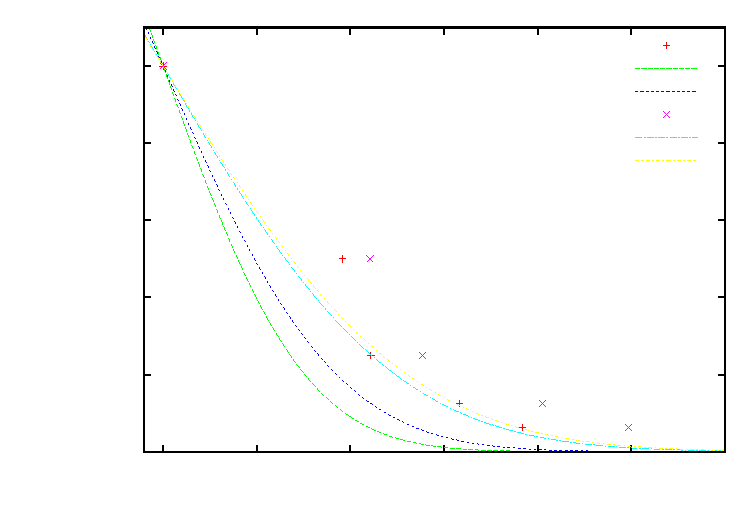
\includegraphics{Diffprofil}}%
    \gplfronttext
  \end{picture}%
\endgroup

	\caption{???????????????????}
\end{figure}

\section{Diskussion}
\label{sec:diskussion}

\section{Anhang}

\begin{thebibliography}{100}

\bibitem{lp} 
	\emph{Lehrportal der Universität Göttingen, Diffusion},
  http://lp.uni-goettingen.de/get/text/3665, abgerufen 09.07.14 11:21 Uhr

\bibitem{gerthsen}
	\textsc{Dieter Meschede} (2010): \emph{Gerthsen Physik}, 24. Auflage, Springer Heidelberg
Dordrecht London New York

\end{thebibliography}

\end{document}
